\documentclass[12pt,a4paper]{article}

% ── Packages ──────────────────────────────────────────────────────────────────
\usepackage[margin=1in]{geometry}
\usepackage{amsmath, amssymb, amsthm}
\usepackage{mathtools}
\usepackage{xcolor}
\usepackage{tcolorbox}
\usepackage{tikz}
\usetikzlibrary{arrows.meta, positioning, shapes.geometric, fit, backgrounds,
                decorations.pathreplacing, calc, automata}
\usepackage{algorithm}
\usepackage{algpseudocode}
\usepackage{hyperref}
\usepackage{enumitem}
\usepackage{fancyhdr}
\usepackage{titlesec}
\usepackage{mdframed}
\usepackage{booktabs}
\usepackage{array}
\usepackage{multirow}
\usepackage{forest}
\usepackage{graphicx}
\usepackage{wrapfig}

% ── Colours ───────────────────────────────────────────────────────────────────
\definecolor{darkblue}{RGB}{0,51,102}
\definecolor{medblue}{RGB}{30,100,180}
\definecolor{lightblue}{RGB}{210,230,255}
\definecolor{darkorange}{RGB}{180,80,0}
\definecolor{lightorange}{RGB}{255,240,210}
\definecolor{darkgreen}{RGB}{0,100,50}
\definecolor{lightgreen}{RGB}{210,245,220}
\definecolor{darkred}{RGB}{150,0,0}
\definecolor{lightred}{RGB}{255,220,220}
\definecolor{lightgray}{RGB}{245,245,245}
\definecolor{midgray}{RGB}{180,180,180}

% ── tcolorbox styles ──────────────────────────────────────────────────────────
\tcbuselibrary{theorems, skins, breakable, listings}

\newtcolorbox{definitionbox}[1][]{
  enhanced, breakable,
  colback=lightblue, colframe=darkblue, colbacktitle=darkblue,
  fonttitle=\bfseries\color{white}, title={#1},
  arc=4pt, boxrule=1.2pt, left=6pt, right=6pt, top=4pt, bottom=4pt
}

\newtcolorbox{theorembox}[1][]{
  enhanced, breakable,
  colback=lightgreen, colframe=darkgreen, colbacktitle=darkgreen,
  fonttitle=\bfseries\color{white}, title={#1},
  arc=4pt, boxrule=1.2pt, left=6pt, right=6pt, top=4pt, bottom=4pt
}

\newtcolorbox{examplebox}[1][]{
  enhanced, breakable,
  colback=lightorange, colframe=darkorange, colbacktitle=darkorange,
  fonttitle=\bfseries\color{white}, title={#1},
  arc=4pt, boxrule=1.2pt, left=6pt, right=6pt, top=4pt, bottom=4pt
}

\newtcolorbox{warningbox}[1][]{
  enhanced, breakable,
  colback=lightred, colframe=darkred, colbacktitle=darkred,
  fonttitle=\bfseries\color{white}, title={#1},
  arc=4pt, boxrule=1.2pt, left=6pt, right=6pt, top=4pt, bottom=4pt
}

\newtcolorbox{intuitionbox}[1][Intuition]{
  enhanced, breakable,
  colback=lightgray, colframe=midgray, colbacktitle=gray,
  fonttitle=\bfseries\color{white}, title={#1},
  arc=4pt, boxrule=1pt, left=6pt, right=6pt
}

% ── Theorem environments ──────────────────────────────────────────────────────
\theoremstyle{plain}
\newtheorem{theorem}{Theorem}[section]
\newtheorem{lemma}[theorem]{Lemma}
\newtheorem{corollary}[theorem]{Corollary}
\newtheorem{proposition}[theorem]{Proposition}

\theoremstyle{definition}
\newtheorem{definition}[theorem]{Definition}
\newtheorem{example}[theorem]{Example}
\newtheorem{exercise}{Exercise}[section]

\theoremstyle{remark}
\newtheorem{remark}[theorem]{Remark}
\newtheorem{note}[theorem]{Note}

% ── Header / footer ───────────────────────────────────────────────────────────
\pagestyle{fancy}
\fancyhf{}
\fancyhead[L]{\small\color{darkblue}\textbf{Lecture Notes: Savitch's Theorem}}
\fancyhead[R]{\small\color{darkblue}Theory of Computation}
\fancyfoot[C]{\thepage}
\renewcommand{\headrulewidth}{0.6pt}

% ── Section colours ───────────────────────────────────────────────────────────
\titleformat{\section}{\large\bfseries\color{darkblue}}{\thesection}{0.8em}{}[\color{darkblue}\titlerule]
\titleformat{\subsection}{\normalsize\bfseries\color{medblue}}{\thesubsection}{0.6em}{}

% ── Macros ────────────────────────────────────────────────────────────────────
\newcommand{\SPACE}{\mathsf{SPACE}}
\newcommand{\NSPACE}{\mathsf{NSPACE}}
\newcommand{\PSPACE}{\mathsf{PSPACE}}
\newcommand{\NPSPACE}{\mathsf{NPSPACE}}
\newcommand{\NL}{\mathsf{NL}}
\newcommand{\coNL}{\mathsf{coNL}}
\newcommand{\LL}{\mathsf{L}}
\newcommand{\NP}{\mathsf{NP}}
\newcommand{\PP}{\mathsf{P}}
\newcommand{\TIME}{\mathsf{TIME}}
\newcommand{\NTIME}{\mathsf{NTIME}}
\newcommand{\poly}{\mathrm{poly}}

% ── Document ──────────────────────────────────────────────────────────────────
\begin{document}

% ── Title page ────────────────────────────────────────────────────────────────
\begin{titlepage}
\centering
\vspace*{2cm}

{\color{darkblue}\rule{\linewidth}{2pt}}
\vspace{0.5cm}

{\Huge\bfseries\color{darkblue} Savitch's Theorem}\\[0.4cm]
{\Large\color{medblue} Space Complexity and the Power of Nondeterminism}\\[0.2cm]
{\color{darkblue}\rule{\linewidth}{2pt}}

\vspace{1.5cm}

\begin{tcolorbox}[colback=lightblue, colframe=darkblue, width=0.85\textwidth,
                  arc=6pt, boxrule=1.5pt]
\centering\large
\textbf{Course:} Theory of Computation\\[4pt]
\textbf{Topic:} Space Complexity Classes\\[4pt]
\textbf{Level:} Undergraduate (Year 3--4)\\[4pt]
\textbf{Prerequisites:} Turing Machines, Basic Complexity, NP-completeness
\end{tcolorbox}

\vspace{2cm}

% ── Conceptual diagram on title page ──────────────────────────────────────────
\begin{tikzpicture}[scale=1.1]
  % Concentric ovals representing class containments
  \fill[lightblue!60]  (0,0) ellipse (5.5cm and 3.2cm);
  \fill[lightgreen!70] (0,0) ellipse (4.2cm and 2.4cm);
  \fill[lightorange!80](0,0) ellipse (3.0cm and 1.7cm);
  \fill[lightred!70]   (0,0) ellipse (1.8cm and 1.0cm);

  \node at (0,0)      {\textbf{\NL}};
  \node at (0,-1.35)  {\textbf{\PP}};
  \node at (0,-1.95)  {\textbf{\NP}};
  \node at (0,-2.6)   {\textbf{\PSPACE = \NPSPACE}};
  \node at (0,-3.5)   {\footnotesize (Savitch: \NPSPACE $\subseteq$ \PSPACE)};

  \draw[darkblue, thick] (0,0) ellipse (5.5cm and 3.2cm);
  \draw[darkgreen, thick](0,0) ellipse (4.2cm and 2.4cm);
  \draw[darkorange, thick](0,0) ellipse (3.0cm and 1.7cm);
  \draw[darkred, thick]  (0,0) ellipse (1.8cm and 1.0cm);
\end{tikzpicture}

\vspace{1.5cm}
{\large\itshape ``Nondeterminism helps much less for space than for time.''}

\vfill
\end{titlepage}

% ── Table of contents ─────────────────────────────────────────────────────────
\tableofcontents
\newpage

% ══════════════════════════════════════════════════════════════════════════════
\section{Introduction and Motivation}
% ══════════════════════════════════════════════════════════════════════════════

\subsection{Why Study Space Complexity?}

So far in your complexity theory journey you have probably spent a lot of time thinking about \emph{time}: how many steps does a Turing machine need to solve a problem? Today we shift perspective to \emph{space}: how much \textbf{memory} (tape cells) does a Turing machine need?

\begin{intuitionbox}
Think of it this way. Imagine you are solving a large puzzle:
\begin{itemize}
  \item \textbf{Time complexity} = how many moves you make.
  \item \textbf{Space complexity} = how much table surface you need to lay out the pieces.
\end{itemize}
These two resources behave very differently!
\end{intuitionbox}

One of the most striking facts in complexity theory is that \textbf{nondeterminism adds much less power for space than it does for time}. For time, we believe $\PP \neq \NP$ — nondeterminism seems to give an exponential advantage. For space, Savitch's theorem shows that nondeterminism gives \emph{at most a quadratic overhead}. This is a profound and beautiful result.

\subsection{A Concrete Motivating Problem: Graph Reachability}

\begin{examplebox}[Example 1.1 — Graph Reachability (ST-CONNECTIVITY)]
\textbf{Problem:} Given a directed graph $G$ and two vertices $s$ and $t$, is there a directed path from $s$ to $t$?

\medskip
\begin{center}
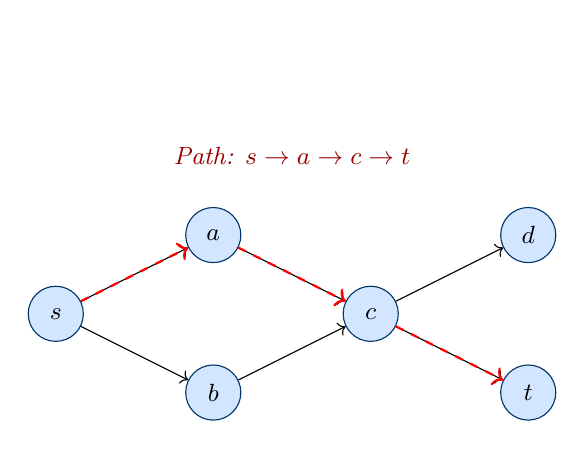
\begin{tikzpicture}[
  node distance=1.8cm,
  every node/.style={circle, draw=darkblue, fill=lightblue, minimum size=0.7cm, font=\small\bfseries},
  every edge/.style={draw=darkblue, -Stealth, thick}
]
  \node (s) at (0,0) {$s$};
  \node (a) at (2,1)  {$a$};
  \node (b) at (2,-1) {$b$};
  \node (c) at (4,0)  {$c$};
  \node (d) at (6,1)  {$d$};
  \node (t) at (6,-1) {$t$};

  \draw[->] (s) -- (a);
  \draw[->] (s) -- (b);
  \draw[->] (a) -- (c);
  \draw[->] (b) -- (c);
  \draw[->] (c) -- (d);
  \draw[->] (c) -- (t);
  \draw[->, dashed, red, thick] (s) -- (a);
  \draw[->, dashed, red, thick] (a) -- (c);
  \draw[->, dashed, red, thick] (c) -- (t);

  \node[draw=none, fill=none, font=\small\itshape, text=darkred] at (3, 2.0) {Path: $s \to a \to c \to t$};
\end{tikzpicture}
\end{center}

\medskip
\textbf{How much space does this need?}
\begin{itemize}
  \item \emph{Nondeterministically:} just guess the next node on the path one step at a time! We only need to remember our \textbf{current position} — that's $O(\log n)$ space (just an index into the vertex list).
  \item \emph{Deterministically:} naive DFS/BFS needs $O(n)$ space to store visited sets.
\end{itemize}
So the nondeterministic algorithm uses far less space. Can a deterministic algorithm do better than $O(n)$?\\
\textbf{Savitch's theorem says yes: $O(\log^2 n)$ space suffices deterministically!}
\end{examplebox}

% ══════════════════════════════════════════════════════════════════════════════
\section{Background: Space Complexity Classes}
% ══════════════════════════════════════════════════════════════════════════════

\subsection{Turing Machine Model for Space}

We use a \textbf{two-tape Turing machine}:
\begin{itemize}
  \item \textbf{Read-only input tape}: contains the input $x$; we do not count this toward space.
  \item \textbf{Read/write work tape}: this is where we count space usage.
\end{itemize}

\begin{center}
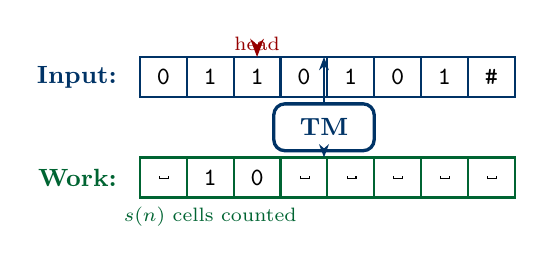
\begin{tikzpicture}[scale=0.85]
  % Input tape
  \foreach \i/\c in {0/0,1/1,2/1,3/0,4/1,5/0,6/1,7/\#} {
    \draw[darkblue, thick] (\i*0.7, 2) rectangle (\i*0.7+0.7, 2.6);
    \node at (\i*0.7+0.35, 2.3) {\small\texttt{\c}};
  }
  \node[darkblue, left] at (-0.2, 2.3) {\small\textbf{Input:}};
  \node[darkred] at (2*0.7+0.35, 2.8) {\scriptsize head};
  \draw[-Stealth, darkred, thick] (2*0.7+0.35, 2.65) -- (2*0.7+0.35, 2.6);

  % Work tape
  \foreach \i/\c in {0/\textvisiblespace,1/1,2/0,3/\textvisiblespace,4/\textvisiblespace,5/\textvisiblespace,6/\textvisiblespace,7/\textvisiblespace} {
    \draw[darkgreen, thick] (\i*0.7, 0.5) rectangle (\i*0.7+0.7, 1.1);
    \node at (\i*0.7+0.35, 0.8) {\small\texttt{\c}};
  }
  \node[darkgreen, left] at (-0.2, 0.8) {\small\textbf{Work:}};
  \draw[darkgreen, thick, dashed] (0,0.5) rectangle (2.1, 1.1);
  \node[darkgreen, below, font=\scriptsize] at (1.05, 0.5) {$s(n)$ cells counted};

  % TM box
  \draw[darkblue, very thick, rounded corners] (2.0, 1.2) rectangle (3.5, 1.9);
  \node[darkblue, font=\small\bfseries] at (2.75, 1.55) {TM};
  \draw[-Stealth, darkblue] (2.75,1.9) -- (2.75, 2.6);
  \draw[-Stealth, darkblue] (2.75,1.2) -- (2.75, 1.1);
\end{tikzpicture}
\end{center}

\begin{definitionbox}[Definition 2.1 — Space Complexity]
Let $M$ be a Turing machine and $x$ be an input. The \textbf{space used by $M$ on $x$}, written $\text{space}_M(x)$, is the number of work-tape cells $M$ visits during its computation on $x$.

The \textbf{space complexity} of $M$ is $s(n) = \max_{|x|=n} \text{space}_M(x)$.

For a \textbf{nondeterministic} TM, we take the maximum over all branches.
\end{definitionbox}

\subsection{The Main Space Complexity Classes}

\begin{definitionbox}[Definition 2.2 — Space Classes]
For a function $s : \mathbb{N} \to \mathbb{N}$:
\[
  \SPACE(s(n)) = \{\,L \mid \text{some \emph{deterministic} TM decides } L \text{ using } O(s(n)) \text{ space}\,\}
\]
\[
  \NSPACE(s(n)) = \{\,L \mid \text{some \emph{nondeterministic} TM decides } L \text{ using } O(s(n)) \text{ space}\,\}
\]

\medskip
Key named classes:
\begin{center}
\renewcommand{\arraystretch}{1.4}
\begin{tabular}{llll}
\toprule
\textbf{Class} & \textbf{Definition} & \textbf{Informal} & \textbf{Example problem}\\
\midrule
$\LL$      & $\SPACE(\log n)$      & Det.\ log space   & Even-length strings \\
$\NL$      & $\NSPACE(\log n)$     & Nondет.\ log space & ST-Connectivity\\
$\PSPACE$  & $\bigcup_k \SPACE(n^k)$ & Det.\ poly space & TQBF, PSPACE-complete\\
$\NPSPACE$ & $\bigcup_k \NSPACE(n^k)$ & Nondet.\ poly space & ---\\
\bottomrule
\end{tabular}
\end{center}
\end{definitionbox}

\begin{intuitionbox}[Why $\log n$ space?]
With $O(\log n)$ bits we can store a counter up to $n$, or an index into the input. This is the minimum nontrivial amount of space (we at least need to remember \emph{where} we are in the input). Problems solvable in $O(\log n)$ space are often those where we only need to keep track of a constant number of pointers or small integers.
\end{intuitionbox}

\subsection{Known Relationships Before Savitch}

Before Savitch's 1970 paper, people knew:
\[
  \LL \subseteq \NL \subseteq \PP \subseteq \NP \subseteq \PSPACE \subseteq \text{EXP}
\]
But the question ``does $\NSPACE(s(n)) = \SPACE(s(n))$?'' was wide open for polynomial $s$.

% ══════════════════════════════════════════════════════════════════════════════
\section{The Key Tool: Reachability in Configuration Graphs}
% ══════════════════════════════════════════════════════════════════════════════

\subsection{Configuration Graphs of Turing Machines}

To prove Savitch's theorem, we need to think of a nondeterministic computation as a \textbf{graph reachability problem}.

\begin{definitionbox}[Definition 3.1 — Configuration]
A \textbf{configuration} of a TM $M$ on input $x$ is a complete description of its current computation state:
\[
  C = (\text{state } q,\ \text{work-tape content},\ \text{position of work-tape head},\ \text{position of input head})
\]
\end{definitionbox}

\begin{examplebox}[Example 3.1 — Visualising Configurations]
Suppose our TM is in state $q_3$, the work tape contains ``\texttt{01}'' with the head over the second cell, and the input head is at position 4. We write this concisely as:
\[
  C = (q_3,\ \texttt{0}\underbrace{1}_{\text{head}},\ \text{input pos}=4)
\]
\end{examplebox}

\begin{definitionbox}[Definition 3.2 — Configuration Graph]
The \textbf{configuration graph} $G_M(x)$ of machine $M$ on input $x$ is a directed graph where:
\begin{itemize}
  \item \textbf{Vertices} = all possible configurations of $M$ on $x$
  \item \textbf{Edges}: there is an edge $C \to C'$ if configuration $C'$ is reachable from $C$ in one step of $M$
\end{itemize}
Let $C_{\text{start}}$ be the initial configuration and $C_{\text{accept}}$ be an accepting configuration.

\medskip
\textbf{Key insight:} $M$ accepts $x$ $\iff$ there is a path from $C_{\text{start}}$ to $C_{\text{accept}}$ in $G_M(x)$.
\end{definitionbox}

\subsection{Size of the Configuration Graph}

\begin{lemma}\label{lem:config-count}
If $M$ uses $s(n)$ space (where $s(n) \geq \log n$), the number of distinct configurations on input of length $n$ is at most
\[
  N = |Q| \cdot n \cdot |\Gamma|^{s(n)} \cdot s(n) \leq c^{s(n)}
\]
for some constant $c$ depending on $M$.
\end{lemma}

\begin{proof}
\begin{itemize}
  \item $|Q|$ choices for the state ($|Q|$ is a constant for a fixed $M$).
  \item $n$ choices for the input head position.
  \item $|\Gamma|^{s(n)}$ choices for the work tape content.
  \item $s(n)$ choices for the work head position.
\end{itemize}
So the total is $|Q| \cdot n \cdot |\Gamma|^{s(n)} \cdot s(n)$. Since $n \leq 2^{s(n)}$ (because $s(n) \geq \log n$), this is at most $(|Q| \cdot |\Gamma| \cdot s(n))^{s(n)} \leq c^{s(n)}$ for large enough constant $c$.
\end{proof}

\begin{center}
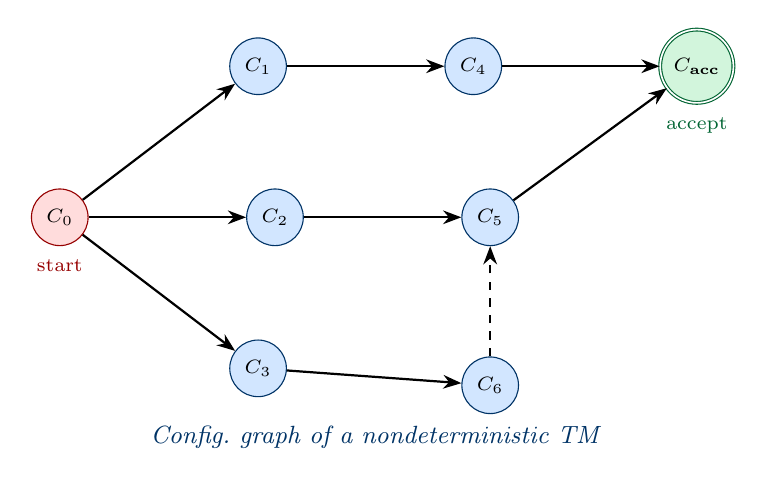
\begin{tikzpicture}[
  node distance=1.4cm and 2cm,
  state/.style={circle, draw=darkblue, fill=lightblue, minimum size=0.65cm, font=\scriptsize\bfseries},
  accept/.style={circle, draw=darkgreen, fill=lightgreen, minimum size=0.65cm, font=\scriptsize\bfseries, double},
  start/.style={circle, draw=darkred, fill=lightred, minimum size=0.65cm, font=\scriptsize\bfseries}
]
\node[start]   (s)  {$C_0$};
\node[state]   (a)  [above right=of s]  {$C_1$};
\node[state]   (b)  [right=of s]        {$C_2$};
\node[state]   (c)  [below right=of s]  {$C_3$};
\node[state]   (d)  [right=of a]        {$C_4$};
\node[state]   (e)  [right=of b]        {$C_5$};
\node[accept]  (f)  [right=of d]        {$C_{\text{acc}}$};
\node[state]   (g)  [below=of e]        {$C_6$};

\draw[-Stealth, thick] (s) -- (a);
\draw[-Stealth, thick] (s) -- (b);
\draw[-Stealth, thick] (s) -- (c);
\draw[-Stealth, thick] (a) -- (d);
\draw[-Stealth, thick] (b) -- (e);
\draw[-Stealth, thick] (c) -- (g);
\draw[-Stealth, thick] (d) -- (f);
\draw[-Stealth, thick] (e) -- (f);
\draw[-Stealth, thick, dashed] (g) -- (e);

\node[font=\scriptsize, darkred, below=0.05cm of s] {start};
\node[font=\scriptsize, darkgreen, below=0.05cm of f] {accept};

\node[font=\small\itshape, text=darkblue] at (4, -2.8)
  {Config.\ graph of a nondeterministic TM};
\end{tikzpicture}
\end{center}

% ══════════════════════════════════════════════════════════════════════════════
\section{Savitch's Theorem}
% ══════════════════════════════════════════════════════════════════════════════

\subsection{Statement of the Theorem}

\begin{theorembox}[Theorem 4.1 — Savitch's Theorem (1970)]
For any function $s(n) \geq \log n$:
\[
  \boxed{\NSPACE(s(n)) \subseteq \SPACE\!\bigl(s(n)^2\bigr)}
\]
In words: \emph{anything solvable by a nondeterministic TM in space $s(n)$ can also be solved by a deterministic TM in space $s(n)^2$.}

\medskip
\textbf{Important corollaries:}
\[
  \PSPACE = \NPSPACE \qquad \text{and} \qquad \NL \subseteq \SPACE(\log^2 n)
\]
\end{theorembox}

\begin{intuitionbox}[Big-Picture Intuition]
The trick is to reduce the acceptance question for a nondeterministic TM to a \textbf{graph reachability problem} on the configuration graph, and then solve that reachability problem \emph{recursively} in a way that uses little space.

The key subroutine: \texttt{REACH}$(C_1, C_2, k)$ = ``Is there a path of length $\leq 2^k$ from config $C_1$ to config $C_2$?''

We solve it by trying all \emph{midpoints} $C_m$: check if $C_1 \xrightarrow{\leq 2^{k-1}} C_m \xrightarrow{\leq 2^{k-1}} C_2$.

The recursion halves $k$ each time, giving depth $O(s(n))$, with each frame using $O(s(n))$ space. Total: $O(s(n)^2)$.
\end{intuitionbox}

\subsection{The Core Algorithm: REACH}

\begin{definitionbox}[Definition 4.1 — The REACH Predicate]
For configurations $C_1$, $C_2$ of a nondeterministic TM $M$, and an integer $k \geq 0$:
\[
  \texttt{REACH}(C_1, C_2, k) = \begin{cases}
    \texttt{true}  & \text{if there is a path } C_1 \to \cdots \to C_2 \text{ of length } \leq 2^k \\
    \texttt{false} & \text{otherwise}
  \end{cases}
\]
\end{definitionbox}

\begin{examplebox}[Example 4.1 — What REACH is doing]
Imagine a sequence of configurations (a path in the configuration graph):
\[
  C_1 \to C_a \to C_b \to \underbrace{C_m}_{\text{midpoint}} \to C_c \to C_d \to C_2
\]
\texttt{REACH}$(C_1, C_2, k)$ asks: is there such a path of length $\leq 2^k$?

The idea is: there exists a midpoint $C_m$ such that
\[
  \texttt{REACH}(C_1, C_m, k{-}1) \;\text{ AND }\; \texttt{REACH}(C_m, C_2, k{-}1)
\]
We just need to \emph{try all possible midpoints} $C_m$.

\begin{center}
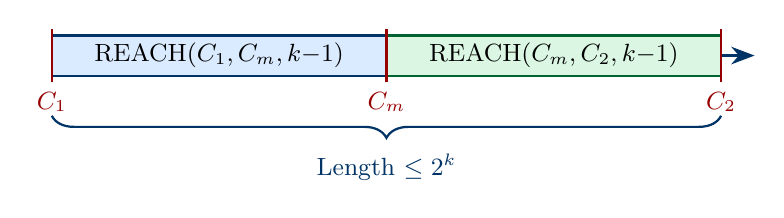
\begin{tikzpicture}[scale=0.85]
  % Timeline
  \draw[darkblue, very thick, -Stealth] (0,0) -- (10.5,0);

  % Blocks
  \fill[lightblue!80] (0,-0.3) rectangle (5.0,0.3);
  \fill[lightgreen!80] (5.0,-0.3) rectangle (10.0,0.3);

  \draw[darkblue, thick] (0,-0.3) rectangle (5.0,0.3);
  \draw[darkgreen, thick] (5.0,-0.3) rectangle (10.0,0.3);

  \node at (2.5, 0) {\small REACH$(C_1, C_m, k{-}1)$};
  \node at (7.5, 0) {\small REACH$(C_m, C_2, k{-}1)$};

  \foreach \x/\l in {0/$C_1$, 5.0/$C_m$, 10.0/$C_2$} {
    \draw[darkred, thick] (\x, -0.4) -- (\x, 0.4);
    \node[darkred, below] at (\x, -0.4) {\small\l};
  }

  \draw[decorate, decoration={brace, amplitude=8pt, mirror}, darkblue, thick]
    (0,-0.9) -- (10.0,-0.9) node[midway, below=10pt] {\small Length $\leq 2^k$};
\end{tikzpicture}
\end{center}
\end{examplebox}

\subsection{The Full Algorithm}

\begin{algorithm}[H]
\caption{\textsc{Reach}$(C_1, C_2, k)$ — Does a path of length $\leq 2^k$ exist from $C_1$ to $C_2$?}
\begin{algorithmic}[1]
\If{$k = 0$}
  \State \Return ($C_1 = C_2$) \textbf{or} ($C_2$ is reachable from $C_1$ in exactly one step)
\EndIf
\For{each configuration $C_m$ (enumerate all $\leq c^{s(n)}$ configurations)}
  \If{\textsc{Reach}$(C_1, C_m, k-1)$ \textbf{and} \textsc{Reach}$(C_m, C_2, k-1)$}
    \State \Return \texttt{true}
  \EndIf
\EndFor
\State \Return \texttt{false}
\end{algorithmic}
\end{algorithm}

\begin{algorithm}[H]
\caption{\textsc{SavitchAccept}$(M, x)$ — Simulate nondeterministic TM $M$ on input $x$}
\begin{algorithmic}[1]
\State $C_{\text{start}} \gets$ initial configuration of $M$ on $x$
\State $C_{\text{acc}} \gets$ accepting configuration of $M$ on $x$
\State $K \gets \lceil \log_2(c^{s(n)}) \rceil = O(s(n))$ \quad\Comment{upper bound on path length}
\State \Return \textsc{Reach}$(C_{\text{start}}, C_{\text{acc}}, K)$
\end{algorithmic}
\end{algorithm}

\subsection{Step-by-Step Example of REACH}

\begin{examplebox}[Example 4.2 — Tracing REACH on a small graph]
Consider this small configuration graph (7 nodes):

\begin{center}
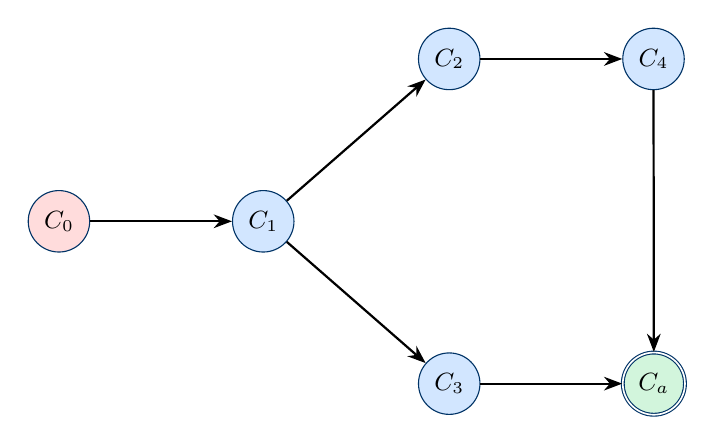
\begin{tikzpicture}[
  node distance=1.5cm and 1.8cm,
  n/.style={circle, draw=darkblue, fill=lightblue, minimum size=0.7cm, font=\small\bfseries}
]
  \node[n, fill=lightred]   (c0) {$C_0$};
  \node[n] (c1) [right=of c0] {$C_1$};
  \node[n] (c2) [above right=of c1] {$C_2$};
  \node[n] (c3) [below right=of c1] {$C_3$};
  \node[n] (c4) [right=of c2] {$C_4$};
  \node[n, fill=lightgreen, double] (ca) [right=of c3] {$C_a$};

  \draw[-Stealth, thick] (c0) -- (c1);
  \draw[-Stealth, thick] (c1) -- (c2);
  \draw[-Stealth, thick] (c1) -- (c3);
  \draw[-Stealth, thick] (c2) -- (c4);
  \draw[-Stealth, thick] (c3) -- (ca);
  \draw[-Stealth, thick] (c4) -- (ca);
\end{tikzpicture}
\end{center}

We want to evaluate \textsc{Reach}$(C_0, C_a, 2)$:

\medskip
\noindent\textbf{Call tree:}
\begin{center}
\begin{forest}
for tree={
  draw=darkblue, fill=lightblue, rounded corners,
  font=\scriptsize, minimum width=3.6cm, minimum height=0.5cm,
  l sep=0.8cm, s sep=0.3cm, edge={-Stealth}
}
[ {REACH$(C_0, C_a, 2)$}
  [ {Try $C_m = C_1$:}
    [ {REACH$(C_0, C_1, 1)$ \checkmark}, fill=lightgreen ]
    [ {REACH$(C_1, C_a, 1)$}
      [ {Try $C_m=C_3$:}
        [ {REACH$(C_1,C_3,0)$\checkmark}, fill=lightgreen ]
        [ {REACH$(C_3,C_a,0)$\checkmark}, fill=lightgreen ]
      ]
    ]
  ]
]
\end{forest}
\end{center}

\medskip
\textbf{Result:} \texttt{REACH}$(C_0, C_a, 2) = \texttt{true}$. The path is $C_0 \to C_1 \to C_3 \to C_a$.
\end{examplebox}

% ══════════════════════════════════════════════════════════════════════════════
\section{Proof of Savitch's Theorem}
% ══════════════════════════════════════════════════════════════════════════════

\subsection{Correctness of REACH}

\begin{lemma}\label{lem:correct}
\textsc{Reach}$(C_1, C_2, k)$ returns \texttt{true} if and only if there is a path from $C_1$ to $C_2$ in the configuration graph of length at most $2^k$.
\end{lemma}

\begin{proof}
By induction on $k$.

\textbf{Base case ($k = 0$):} A path of length $\leq 2^0 = 1$ means either $C_1 = C_2$ (path of length 0) or there is a direct edge $C_1 \to C_2$ (path of length 1). The algorithm checks exactly this.

\textbf{Inductive step ($k > 0$):} Assume the result holds for $k - 1$. We want to show it holds for $k$.

($\Rightarrow$) Suppose \textsc{Reach}$(C_1, C_2, k)$ returns \texttt{true}. Then for some midpoint $C_m$, both \textsc{Reach}$(C_1, C_m, k-1)$ and \textsc{Reach}$(C_m, C_2, k-1)$ return \texttt{true}. By the induction hypothesis, there are paths $C_1 \rightsquigarrow C_m$ of length $\leq 2^{k-1}$ and $C_m \rightsquigarrow C_2$ of length $\leq 2^{k-1}$. Concatenating gives a path $C_1 \rightsquigarrow C_2$ of length $\leq 2^{k-1} + 2^{k-1} = 2^k$.

($\Leftarrow$) Suppose there is a path $C_1 = D_0, D_1, \ldots, D_\ell = C_2$ with $\ell \leq 2^k$. Let $C_m = D_{\lfloor \ell/2 \rfloor}$ be the midpoint. Then there is a path from $C_1$ to $C_m$ of length $\lfloor \ell/2 \rfloor \leq 2^{k-1}$, and from $C_m$ to $C_2$ of length $\lceil \ell/2 \rceil \leq 2^{k-1}$. By induction, both recursive calls return \texttt{true}. So when the algorithm tries $C_m$, it returns \texttt{true}.
\end{proof}

\subsection{Space Analysis — The Heart of the Proof}

This is the most important and subtle part. We need to show that \textsc{Reach} uses only $O(s(n)^2)$ space.

\begin{warningbox}[Common Misconception!]
Students often worry: ``If we recurse to depth $O(s(n))$, and each level tries all $c^{s(n)}$ midpoints, don't we need exponential space to store all those attempts?''

\textbf{No!} The key insight is that we try each midpoint $C_m$ \emph{one at a time}, and reuse space. We never need to store multiple midpoints simultaneously.
\end{warningbox}

\begin{proof}[Proof of Space Bound]
We analyze the space used by the recursive call stack.

\textbf{Space per stack frame:} Each call to \textsc{Reach}$(C_1, C_2, k)$ stores:
\begin{itemize}
  \item $C_1$: a configuration, taking $O(s(n))$ space.
  \item $C_2$: a configuration, taking $O(s(n))$ space.
  \item $k$: an integer $\leq s(n)$, taking $O(\log s(n)) = O(s(n))$ space.
  \item $C_m$: the current midpoint being tried, $O(s(n))$ space.
\end{itemize}
Total per frame: $O(s(n))$.

\textbf{Recursion depth:} Starting with $k = O(s(n))$, each recursive call decrements $k$ by 1. The maximum recursion depth is $O(s(n))$.

\textbf{Crucial point — reuse of space:} When we call \textsc{Reach}$(C_1, C_m, k-1)$, we don't need to keep $C_m$ active for the second call \textsc{Reach}$(C_m, C_2, k-1)$ because:
\begin{enumerate}
  \item We first compute \textsc{Reach}$(C_1, C_m, k-1)$.
  \item If it returns \texttt{true}, we \emph{remember} $C_m$ (it's on the current stack frame) and then compute \textsc{Reach}$(C_m, C_2, k-1)$.
  \item The two recursive calls happen \emph{sequentially}, not simultaneously, so only one branch of the recursion is alive at any point.
\end{enumerate}
This means the stack looks like:

\begin{center}
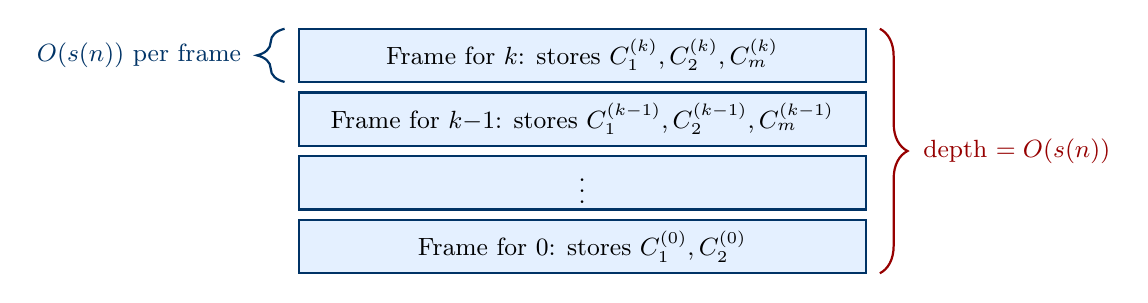
\begin{tikzpicture}[scale=0.9]
  \foreach \i/\l in {0/{\small Frame for $k$: stores $C_1^{(k)}, C_2^{(k)}, C_m^{(k)}$},
                      1/{\small Frame for $k{-}1$: stores $C_1^{(k-1)}, C_2^{(k-1)}, C_m^{(k-1)}$},
                      2/{\small $\vdots$},
                      3/{\small Frame for $0$: stores $C_1^{(0)}, C_2^{(0)}$}} {
    \draw[darkblue, thick, fill=lightblue!60] (0, -\i*0.9) rectangle (8, -\i*0.9+0.75);
    \node[font=\small] at (4, -\i*0.9+0.38) {\l};
  }
  \draw[decorate, decoration={brace, amplitude=10pt}, darkred, thick]
    (8.2, 0.75) -- (8.2, -3*0.9) node[midway, right=12pt, font=\small] {depth $= O(s(n))$};
  \draw[decorate, decoration={brace, amplitude=10pt, mirror}, darkblue, thick]
    (-0.2, 0.75) -- (-0.2, 0) node[midway, left=12pt, font=\small] {$O(s(n))$ per frame};
\end{tikzpicture}
\end{center}

\textbf{Total space:}
\[
  O(s(n)) \text{ space per frame} \;\times\; O(s(n)) \text{ depth} \;=\; O(s(n)^2)
\]

This completes the proof that the deterministic simulation uses $O(s(n)^2)$ space.
\end{proof}

\subsection{Putting It All Together}

\begin{proof}[Proof of Savitch's Theorem]
Let $L \in \NSPACE(s(n))$. Then there is a nondeterministic TM $N$ that decides $L$ using space $O(s(n))$.

We build a deterministic TM $M$ that decides $L$ as follows:
\begin{enumerate}
  \item On input $x$ of length $n$, $M$ computes $C_{\text{start}}$ and $C_{\text{acc}}$ for $N$ on $x$.
  \item $M$ runs algorithm \textsc{Reach}$(C_{\text{start}}, C_{\text{acc}}, K)$ where $K = \lceil c \cdot s(n) \rceil$ for constant $c$ large enough that $2^K$ exceeds the number of configurations of $N$ on $x$.
  \item $M$ accepts iff \textsc{Reach} returns \texttt{true}.
\end{enumerate}

\textbf{Correctness:} By Lemma~\ref{lem:correct} and the fact that $N$ accepts $x$ iff $C_{\text{acc}}$ is reachable in the configuration graph.

\textbf{Space:} By the analysis above, the total space is $O(s(n)^2)$.

Therefore $L \in \SPACE(s(n)^2)$, and since $L$ was arbitrary, $\NSPACE(s(n)) \subseteq \SPACE(s(n)^2)$. \qed
\end{proof}

% ══════════════════════════════════════════════════════════════════════════════
\section{Corollaries and Consequences}
% ══════════════════════════════════════════════════════════════════════════════

\subsection{The Big Picture}

\begin{theorembox}[Corollary 5.1 — PSPACE = NPSPACE]
$\PSPACE = \NPSPACE$.
\end{theorembox}
\begin{proof}
Clearly $\PSPACE \subseteq \NPSPACE$. For the other direction:
\[
  \NPSPACE = \bigcup_k \NSPACE(n^k) \;\xrightarrow{\text{Savitch}}\; \bigcup_k \SPACE(n^{2k}) = \PSPACE.
\]
\end{proof}

\begin{theorembox}[Corollary 5.2 — NL is in $\SPACE(\log^2 n)$]
$\NL \subseteq \SPACE(\log^2 n)$.
\end{theorembox}
\begin{proof}
$\NL = \NSPACE(\log n)$. By Savitch's theorem, $\NSPACE(\log n) \subseteq \SPACE((\log n)^2) = \SPACE(\log^2 n)$.
\end{proof}

\begin{remark}
In fact, Immerman and Szelepcs\'{e}nyi (1987, 1988) proved the even stronger result $\NL = \coNL$, meaning nondeterministic log space is closed under complementation. This is another landmark theorem in space complexity.
\end{remark}

\subsection{Updated Class Diagram}

\begin{center}
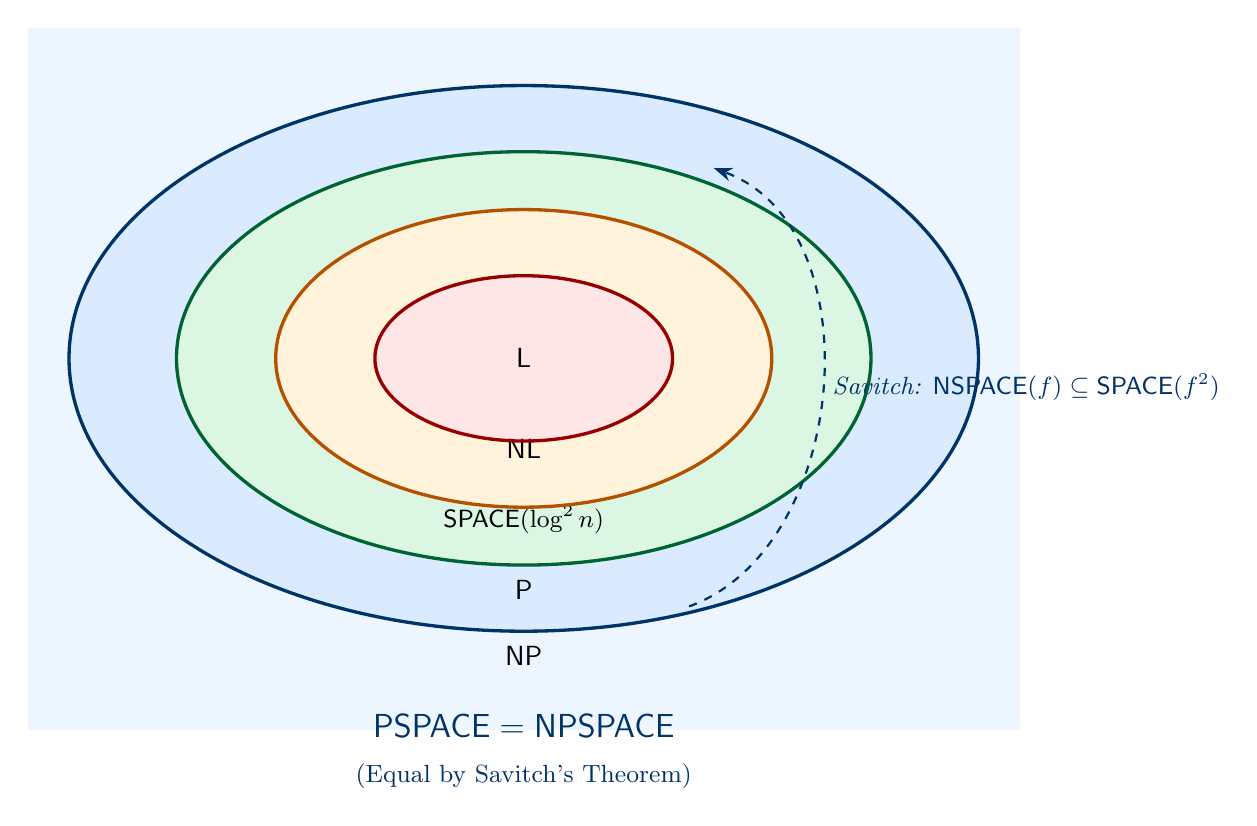
\begin{tikzpicture}[scale=1.05]
  % Regions
  \fill[lightblue!40] (-1,-1) rectangle (11, 7.5);

  \begin{scope}
    \clip (-1,-1) rectangle (11,7.5);
    \fill[lightblue!80]   (5,3.5) ellipse (5.5cm and 3.3cm);
    \fill[lightgreen!80]  (5,3.5) ellipse (4.2cm and 2.5cm);
    \fill[lightorange!80] (5,3.5) ellipse (3.0cm and 1.8cm);
    \fill[lightred!70]    (5,3.5) ellipse (1.8cm and 1.0cm);
  \end{scope}

  % Labels
  \node[font=\bfseries] at (5, 3.5)   {$\LL$};
  \node[font=\bfseries] at (5, 2.4)   {$\NL$};
  \node[font=\small\bfseries] at (5, 1.55)  {$\SPACE(\log^2 n)$};
  \node[font=\bfseries] at (5, 0.7)   {$\PP$};
  \node[font=\bfseries] at (5, -0.1)  {$\NP$};
  \node[font=\bfseries\color{darkblue}] at (5, -0.95) {\large $\PSPACE = \NPSPACE$};

  % Borders
  \draw[darkred, very thick]    (5,3.5) ellipse (1.8cm and 1.0cm);
  \draw[darkorange, very thick] (5,3.5) ellipse (3.0cm and 1.8cm);
  \draw[darkgreen, very thick]  (5,3.5) ellipse (4.2cm and 2.5cm);
  \draw[darkblue, very thick]   (5,3.5) ellipse (5.5cm and 3.3cm);

  % Savitch annotation
  \draw[-Stealth, darkblue, thick, dashed]
    (7, 0.5) to[out=20, in=-20] node[right, font=\small\itshape] {Savitch: $\NSPACE(f) \subseteq \SPACE(f^2)$} (7.3, 5.8);

  \node[font=\small, darkblue] at (5, -1.55) {(Equal by Savitch's Theorem)};
\end{tikzpicture}
\end{center}

\subsection{Comparison: Time vs Space Nondeterminism}

\begin{center}
\renewcommand{\arraystretch}{1.5}
\begin{tabular}{>{\bfseries}l l l}
\toprule
& \textbf{Time} & \textbf{Space} \\
\midrule
Det.\ vs Nondet. & $\PP$ vs $\NP$ (open!) & $\PSPACE = \NPSPACE$ (Savitch!) \\
Overhead known? & Unknown (exp.\ is believed) & At most quadratic \\
Key question & $\PP = \NP$? & Resolved (equal for poly) \\
Log-space & $\LL$ vs $\NL$ (open) & $\NL \subseteq \SPACE(\log^2 n)$ \\
\bottomrule
\end{tabular}
\end{center}

\begin{intuitionbox}[Why is space different from time?]
Space can be \textbf{reused}! Once a Turing machine finishes using a region of tape, it can write over it and reuse that space for something else. Time cannot be reused: once a step is taken, it is gone. This reusability is why space is ``more compressible'' and why nondeterminism helps less.
\end{intuitionbox}

% ══════════════════════════════════════════════════════════════════════════════
\section{Worked Examples and Applications}
% ══════════════════════════════════════════════════════════════════════════════

\subsection{Example: ST-Connectivity in $\SPACE(\log^2 n)$}

\begin{examplebox}[Example 6.1 — ST-CONNECTIVITY $\in \SPACE(\log^2 n)$]
Recall ST-CONNECTIVITY: given directed graph $G=(V,E)$ and vertices $s,t$, is there a path $s \rightsquigarrow t$?

\textbf{Why it's in NL:} A nondeterministic log-space algorithm just guesses the path one vertex at a time. It stores only the current vertex (needs $\log n$ bits) and a step counter (needs $\log n$ bits). Total: $O(\log n)$ space.

\textbf{By Savitch:} ST-CONNECTIVITY $\in \SPACE(\log^2 n)$. The algorithm is exactly \textsc{Reach} from above, applied to the actual graph (not the configuration graph of a TM).

\medskip
\textbf{Concretely}, on a graph with $n=16$ vertices, $\log n = 4$, so $\log^2 n = 16$ bits of workspace — enough to store 2--3 vertex indices and a counter.
\end{examplebox}

\begin{examplebox}[Example 6.2 — Tracing \textsc{Reach} on a Graph]
Graph: $V = \{1,2,3,4,5\}$, edges: $1\to2$, $2\to3$, $3\to4$, $4\to5$. Query: Is $5$ reachable from $1$?

\begin{center}
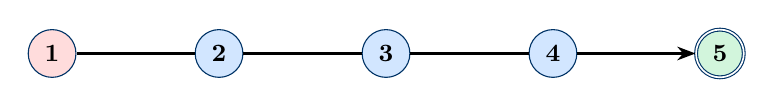
\begin{tikzpicture}[node distance=1.5cm, n/.style={circle,draw=darkblue,fill=lightblue,minimum size=0.6cm,font=\small\bfseries}]
  \node[n,fill=lightred] (1) {1};
  \node[n] (2) [right=of 1] {2};
  \node[n] (3) [right=of 2] {3};
  \node[n] (4) [right=of 3] {4};
  \node[n,fill=lightgreen,double] (5) [right=of 4] {5};
  \draw[-Stealth,thick] (1)--(2)--(3)--(4)--(5);
\end{tikzpicture}
\end{center}

Run \textsc{Reach}$(1, 5, 2)$ (since path length $= 4 = 2^2$, $k=2$ suffices):

\begin{itemize}
  \item Try midpoint $C_m = 3$: \textsc{Reach}$(1,3,1)$?
  \begin{itemize}
    \item Try $C_m = 2$: \textsc{Reach}$(1,2,0)$? $\checkmark$ (direct edge). \textsc{Reach}$(2,3,0)$? $\checkmark$. \textbf{Return true.}
  \end{itemize}
  \item Now \textsc{Reach}$(3,5,1)$?
  \begin{itemize}
    \item Try $C_m = 4$: \textsc{Reach}$(3,4,0)$? $\checkmark$. \textsc{Reach}$(4,5,0)$? $\checkmark$. \textbf{Return true.}
  \end{itemize}
  \item Both halves true $\Rightarrow$ \textsc{Reach}$(1,5,2) = \texttt{true}$. \checkmark
\end{itemize}
\end{examplebox}

\subsection{Example: TQBF is PSPACE-Complete}

\begin{examplebox}[Example 6.3 — TQBF and PSPACE]
The True Quantified Boolean Formula problem (TQBF) asks: is a fully quantified Boolean formula (e.g. $\exists x_1 \forall x_2 \exists x_3 \; \phi(x_1,x_2,x_3)$) true?

\textbf{Facts:}
\begin{itemize}
  \item TQBF $\in \PSPACE$: evaluate quantifiers one by one, reusing space.
  \item TQBF is PSPACE-\emph{complete}: every problem in PSPACE reduces to it.
  \item Since $\PSPACE = \NPSPACE$ (Savitch), TQBF is also NPSPACE-complete.
\end{itemize}

This means TQBF is in some sense the \emph{hardest} problem in PSPACE, just as SAT is the hardest in NP.
\end{examplebox}

\subsection{The Space Hierarchy and Where Savitch Fits}

\begin{center}
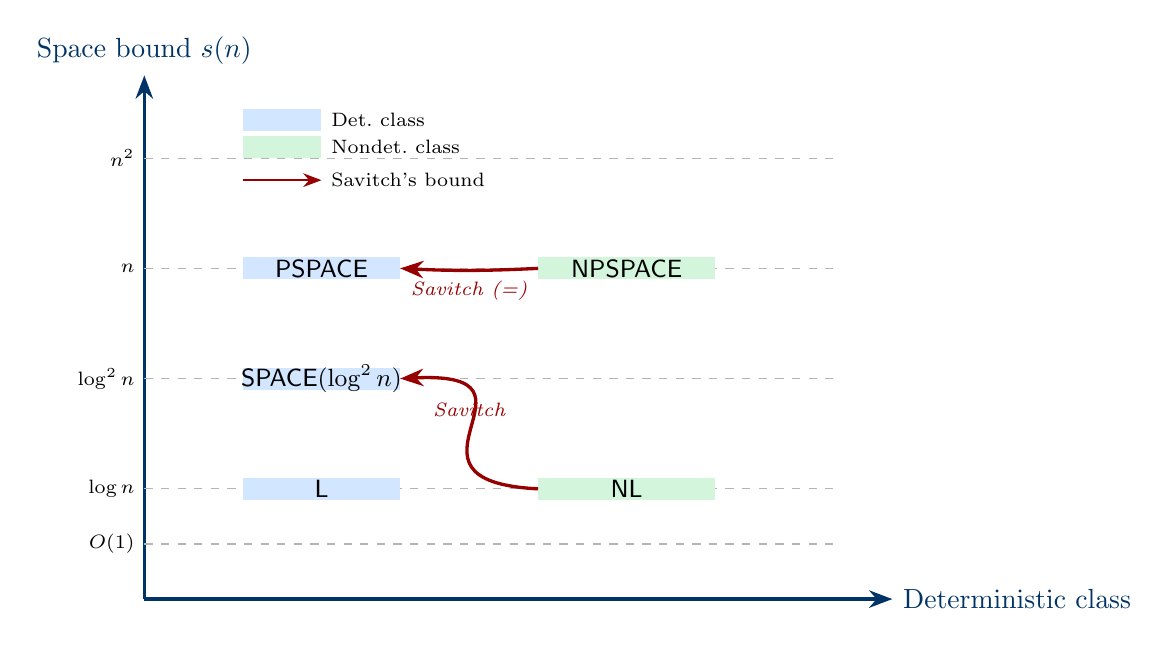
\begin{tikzpicture}[xscale=2.5, yscale=0.7]
  \draw[-Stealth, darkblue, very thick] (0,0) -- (0, 9.5) node[above] {Space bound $s(n)$};
  \draw[-Stealth, darkblue, very thick] (0,0) -- (3.8,0) node[right] {Deterministic class};

  % Grid lines
  \foreach \y/\l in {1/$O(1)$, 2/$\log n$, 4/$\log^2 n$, 6/$n$, 8/$n^2$} {
    \draw[midgray, dashed] (0,\y) -- (3.5,\y);
    \node[left, font=\scriptsize] at (0,\y) {\l};
  }

  % Deterministic classes
  \fill[lightblue] (0.5, 1.8) rectangle (1.3, 2.2);
  \node[font=\small\bfseries] at (0.9, 2.0) {$\LL$};

  \fill[lightblue] (0.5, 3.8) rectangle (1.3, 4.2);
  \node[font=\small\bfseries] at (0.9, 4.0) {$\SPACE(\log^2 n)$};

  \fill[lightblue] (0.5, 5.8) rectangle (1.3, 6.2);
  \node[font=\small\bfseries] at (0.9, 6.0) {$\PSPACE$};

  % Nondeterministic classes
  \fill[lightgreen] (2.0, 1.8) rectangle (2.9, 2.2);
  \node[font=\small\bfseries] at (2.45, 2.0) {$\NL$};

  \fill[lightgreen] (2.0, 5.8) rectangle (2.9, 6.2);
  \node[font=\small\bfseries] at (2.45, 6.0) {$\NPSPACE$};

  % Savitch arrows
  \draw[-Stealth, darkred, very thick]
    (2.0, 2.0) to[out=170, in=10] node[above, font=\scriptsize\itshape, darkred] {Savitch} (1.3, 4.0);

  \draw[-Stealth, darkred, very thick]
    (2.0, 6.0) to[out=190, in=-10] node[below, font=\scriptsize\itshape, darkred] {Savitch (=)} (1.3, 6.0);

  % Legend
  \fill[lightblue] (0.5, 8.5) rectangle (0.9, 8.9); \node[right, font=\scriptsize] at (0.9,8.7) {Det.\ class};
  \fill[lightgreen] (0.5, 8.0) rectangle (0.9, 8.4); \node[right, font=\scriptsize] at (0.9,8.2) {Nondet.\ class};
  \draw[-Stealth,darkred,thick] (0.5,7.6)--(0.9,7.6); \node[right, font=\scriptsize] at (0.9,7.6) {Savitch's bound};
\end{tikzpicture}
\end{center}

% ══════════════════════════════════════════════════════════════════════════════
\section{Why the Quadratic Overhead? Limits of the Technique}
% ══════════════════════════════════════════════════════════════════════════════

\subsection{Is the $s(n)^2$ Tight?}

A natural question: can we do better than $O(s(n)^2)$?

\begin{itemize}
  \item For $\NL$: it is conjectured that $\NL = \LL$ (nondeterminism doesn't help at all for log space), but this is open.
  \item The quadratic overhead in Savitch is an artefact of the divide-and-conquer recursion. Nobody knows if $\NSPACE(f) \subseteq \SPACE(f^{1.5})$ or better in general.
  \item For polynomial space, $\PSPACE = \NPSPACE$ is exact — nondeterminism gives \emph{zero} asymptotic overhead.
\end{itemize}

\subsection{Where Does the $s(n)^2$ Come From?}

\begin{center}
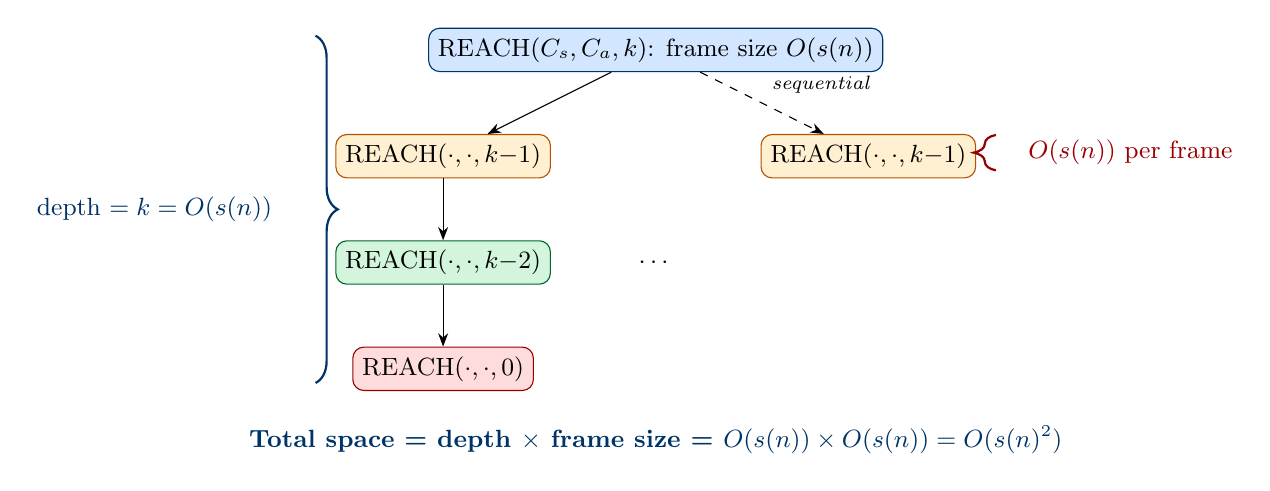
\begin{tikzpicture}[scale=0.9]
  % Call tree showing depth and width
  \node[draw=darkblue, fill=lightblue, rounded corners, font=\small] (root) at (5,6)
    {REACH$(C_s, C_a, k)$: frame size $O(s(n))$};

  \node[draw=darkorange, fill=lightorange, rounded corners, font=\small] (l1a) at (2,4.5)
    {REACH$(\cdot,\cdot, k{-}1)$};
  \node[draw=darkorange, fill=lightorange, rounded corners, font=\small] (l1b) at (8,4.5)
    {REACH$(\cdot,\cdot, k{-}1)$};

  \node[draw=darkgreen, fill=lightgreen, rounded corners, font=\small] (l2) at (2,3)
    {REACH$(\cdot,\cdot, k{-}2)$};
  \node[font=\small] at (5,3) {$\cdots$};

  \node[draw=darkred, fill=lightred, rounded corners, font=\small] (base) at (2,1.5)
    {REACH$(\cdot,\cdot, 0)$};

  \draw[-Stealth] (root) -- (l1a);
  \draw[-Stealth, dashed] (root) -- (l1b) node[midway, above right, font=\scriptsize\itshape]{sequential};
  \draw[-Stealth] (l1a) -- (l2);
  \draw[-Stealth] (l2) -- (base);

  % Depth annotation
  \draw[decorate, decoration={brace, amplitude=8pt, mirror}, darkblue, thick]
    (0.2, 1.3) -- (0.2, 6.2) node[midway, left=12pt, font=\small] {depth $= k = O(s(n))$};

  % Frame annotation
  \draw[decorate, decoration={brace, amplitude=8pt}, darkred, thick]
    (9.8, 4.3) -- (9.8, 4.8) node[midway, right=8pt, font=\small] {$O(s(n))$ per frame};

  \node[font=\small\bfseries, darkblue] at (5, 0.5)
    {Total space = depth $\times$ frame size = $O(s(n)) \times O(s(n)) = O(s(n)^2)$};
\end{tikzpicture}
\end{center}

% ══════════════════════════════════════════════════════════════════════════════
\section{Summary and Key Takeaways}
% ══════════════════════════════════════════════════════════════════════════════

\begin{tcolorbox}[colback=lightblue, colframe=darkblue, colbacktitle=darkblue,
                  fonttitle=\bfseries\color{white}, title={Chapter Summary},
                  arc=4pt, boxrule=1.2pt, breakable]
\begin{enumerate}
  \item \textbf{Savitch's Theorem:} $\NSPACE(s(n)) \subseteq \SPACE(s(n)^2)$ for $s(n) \geq \log n$.
  \item \textbf{Immediate consequence:} $\PSPACE = \NPSPACE$. Nondeterminism gives zero asymptotic overhead for polynomial space!
  \item \textbf{For log space:} $\NL \subseteq \SPACE(\log^2 n)$, though whether $\NL = \LL$ is still open.
  \item \textbf{Key technique:} Convert NTM acceptance to graph reachability, then solve reachability using divide-and-conquer (\textsc{Reach}) with only $O(s(n)^2)$ space by reusing stack frames sequentially.
  \item \textbf{Space vs.\ time:} Nondeterminism is ``cheaper'' in space because space can be reused. Time cannot be rewound.
  \item \textbf{Historical note:} Walter Savitch proved this theorem in 1970. It remains one of the most elegant results in complexity theory.
\end{enumerate}
\end{tcolorbox}

% ══════════════════════════════════════════════════════════════════════════════
\section{Exercises}
% ══════════════════════════════════════════════════════════════════════════════

\begin{exercise}[Warm-up: Space classes]\label{ex:warmup}
Without using Savitch's theorem, show directly that $\SPACE(s(n)) \subseteq \NSPACE(s(n))$ for all $s$. Which direction of the containment does Savitch's theorem address?
\end{exercise}

\begin{exercise}[Configuration counting]\label{ex:configs}
Suppose a nondeterministic TM $N$ has 10 states and uses a work tape alphabet of size 4. On inputs of length $n$, $N$ uses at most $s(n) = 3\log_2 n$ tape cells.
\begin{enumerate}[label=(\alph*)]
  \item Give an upper bound on the number of distinct configurations of $N$ on an input of length $n$.
  \item What is the value of $K$ (the initial value of $k$) needed in \textsc{SavitchAccept}?
  \item For $n = 64$, compute the exact number of configurations using the formula from part (a).
\end{enumerate}
\end{exercise}

\begin{exercise}[Tracing REACH]\label{ex:trace}
Consider the following directed graph:
\[
  V = \{A, B, C, D, E\}, \quad E = \{(A,B),(A,C),(B,D),(C,D),(D,E)\}
\]
\begin{enumerate}[label=(\alph*)]
  \item Draw the graph.
  \item Is $E$ reachable from $A$? What is the shortest path?
  \item Trace the execution of \textsc{Reach}$(A, E, 2)$ step by step, showing which midpoints are tried and which recursive calls are made.
  \item What is the maximum recursion depth reached, and how many recursive calls are made in total?
\end{enumerate}
\end{exercise}

\begin{exercise}[Space analysis]\label{ex:space}
In the proof of Savitch's theorem, we claimed each stack frame uses $O(s(n))$ space.
\begin{enumerate}[label=(\alph*)]
  \item List all the variables stored in a single stack frame of \textsc{Reach}$(C_1, C_2, k)$. How many bits does each require?
  \item Suppose $s(n) = n$. Compute the total space used by \textsc{SavitchAccept} in terms of $n$.
  \item Why is it important that the two recursive calls in \textsc{Reach} are \emph{sequential} rather than \emph{parallel}? What would happen to the space usage if they were parallel?
\end{enumerate}
\end{exercise}

\begin{exercise}[Applying Savitch]\label{ex:apply}
For each of the following problems, determine whether it is in $\SPACE(\log^2 n)$. Justify your answer.
\begin{enumerate}[label=(\alph*)]
  \item \textsc{2-SAT}: Given a CNF formula with at most 2 literals per clause, is it satisfiable?\\
  \textit{Hint:} 2-SAT is NL-complete.
  \item \textsc{UnReach}: Given a graph $G$ and vertices $s, t$, is $t$ \emph{not} reachable from $s$?\\
  \textit{Hint:} This is in coNL. Use the Immerman--Szelepcs\'{e}nyi theorem: $\NL = \text{coNL}$.
  \item \textsc{Graph-Isomorphism}: Are two given graphs isomorphic?\\
  \textit{Hint:} It is not known whether this is in NL.
\end{enumerate}
\end{exercise}

\begin{exercise}[Stronger containment for polynomial space]\label{ex:poly}
Let $f(n) = n^k$ for some fixed integer $k \geq 1$.
\begin{enumerate}[label=(\alph*)]
  \item Apply Savitch's theorem to show $\NSPACE(n^k) \subseteq \SPACE(n^{2k})$.
  \item Conclude that $\NPSPACE \subseteq \PSPACE$.
  \item Why does this give $\PSPACE = \NPSPACE$ (not just $\NPSPACE \subseteq \PSPACE$)?
\end{enumerate}
\end{exercise}

\begin{exercise}[Challenge: Space-time tradeoffs]\label{ex:challenge}
The naive DFS algorithm for ST-CONNECTIVITY on a graph with $n$ vertices and $m$ edges uses $O(n)$ space (to store the visited set). Savitch's algorithm uses $O(\log^2 n)$ space but may be slower.
\begin{enumerate}[label=(\alph*)]
  \item Estimate the \emph{time} complexity of \textsc{SavitchAccept} on an $n$-vertex graph. (Hint: how many recursive calls are made at each level? How many levels are there? How many midpoints are tried at each call?)
  \item Compare: which is faster, DFS or Savitch's algorithm? Which uses less space?
  \item Can you think of a real-world scenario where using Savitch's algorithm (more time, less space) would be preferable to DFS?
\end{enumerate}
\end{exercise}

\begin{exercise}[Conceptual]\label{ex:conceptual}
Answer the following short questions:
\begin{enumerate}[label=(\alph*)]
  \item Savitch's theorem shows $\NSPACE(f) \subseteq \SPACE(f^2)$. Is it believed that the exponent 2 is necessary (i.e., that $\NSPACE(f) \not\subseteq \SPACE(f^{1.99})$ for all $f$)? Explain.
  \item Why is there no analogous theorem for time, i.e., $\NTIME(f) \subseteq \TIME(f^2)$? (Or is there?)
  \item True or false: Savitch's theorem implies $\PP = \NP$. Justify.
\end{enumerate}
\end{exercise}

\appendix
% ══════════════════════════════════════════════════════════════════════════════
\section{Quick Reference}
% ══════════════════════════════════════════════════════════════════════════════

\begin{center}
\renewcommand{\arraystretch}{1.5}
\begin{tabular}{lll}
\toprule
\textbf{Symbol} & \textbf{Meaning} & \textbf{Notes} \\
\midrule
$\SPACE(f)$ & Det.\ TM, space $O(f(n))$ & Work tape only \\
$\NSPACE(f)$ & Nondet.\ TM, space $O(f(n))$ & Max over all branches \\
$\LL$ & $\SPACE(\log n)$ & Log space \\
$\NL$ & $\NSPACE(\log n)$ & Nondet.\ log space \\
$\PSPACE$ & $\bigcup_k \SPACE(n^k)$ & Poly space \\
$\NPSPACE$ & $\bigcup_k \NSPACE(n^k)$ & = PSPACE (Savitch) \\
$C_{\text{start}}$ & Initial TM configuration & \\
$C_{\text{acc}}$ & Accepting TM configuration & \\
\textsc{Reach}$(C_1,C_2,k)$ & Savitch subroutine & Path of length $\leq 2^k$? \\
\bottomrule
\end{tabular}
\end{center}

\subsection{Savitch's Theorem at a Glance}

\begin{tcolorbox}[colback=lightgreen, colframe=darkgreen, arc=6pt, boxrule=1.5pt]
\centering
\Large
\[
  \NSPACE(s(n)) \subseteq \SPACE(s(n)^2) \quad (s(n) \geq \log n)
\]
\normalsize
Proof idea: reduce to graph reachability; solve with divide-and-conquer \textsc{Reach}.\\
Stack depth $O(s(n))$ $\times$ frame size $O(s(n))$ = total space $O(s(n)^2)$.
\end{tcolorbox}

\end{document}
